\documentclass[12pt]{article}
\usepackage{preamble}
\usetikzlibrary{decorations.pathreplacing}
% -- document title --
\title{Impacts of Childcare Service on Mothers' Labor Supply: \\ 
       Evidence from Optional Separate Surnames in Japan\thanks{
        This proposal is not prepared for the thesis, but I plan to use it if the optional separate surname policy is implemented in Japan.
       }
       }
\author{Sakito Tango\thanks{id: 29246024, 
        email: \href{mailto:tango-sakito@g.ecc.u-tokyo.ac.jp}{tango-sakito@g.ecc.u-tokyo.ac.jp}
}
}
\date{\today}
% --------------------------

\begin{document}

\maketitle

\section{Research Question}
This proposal aims to answer the following questions: Do mothers work more if they have better access to childcare services? 
In other words, how large is the treatment effect of childcare services on mothers' labor supply?
To estimate, I suggest using the introduction of optional separate surnames as a natural experiment, which has not been introduced in Japan yet.
The estimation design I use is the randomized assignment with incomplete compliance; the announcement of the introduction of optional separate surnames is the random assignment of treatment, the use of childcare service is the take-up of treatment, and mothers' labor supply is the outcome.
The necessary dataset is the large-scale version of the Comprehensive Survey of Living Conditions, which the Ministry of Health, Labour, and Welfare conducts every three years.


The remainder of this proposal is organized as follows. 
Section 2 motivates this proposal. 
Section 3 explains the potential institutional background of optional separate surnames which I assume in this proposal.
Section 4 formulates the empirical model and explains why the identification strategy is valid.
Section 5 describes the data I use in this proposal.


\section{Motivation}
The relationship between fertility and mothers' labor supply is one of the significant topics in Japan. 
According to the Japanese National Fertility Survey, conducted in 2021 by the National Institute of Population and Social Security Research, about 41\%  of full-time working mothers stop working full-time after the birth of their first child.
Providing an environment where mothers can work while raising children is essential to promote the full use of labor resources, female social advancement, and fertility rate.


In this context, the effectiveness of childcare services is a crucial issue. 
Expanding childcare services is expected to reduce mothers' burden of child-rearing and increase their labor supply.
According to the Children and Families Agency, the supply of childcare services has been increasing. 
However, the capacity fill rate is still around 90\%, which means that the supply is insufficient to meet the demand.
Also, increasing its supply requires a large budget, so evaluating its effectiveness is integral.


A wide range of studies estimate the effect of childcare services on mothers' labor supply.
\cite{Baker2008-vt} is one of the most famous studies. 
They use the introduction of childcare services in Quebec, Canada, and show that the policy increased mothers' labor supply.
Also, \cite{kondo2024} shows that the take-up of accredited childcare services, a primary type of childcare services in Japan, increases mothers' labor supply using an administrative dataset.
However, results on the causal effect are mixed, and one difficulty in estimating the effect is the endogeneity problem.
Mothers who want to work more are likely to be more enthusiastic about applying for childcare services.
Also, it is the government that decides the supply of childcare services. 
The government which increases the supply of childcare services is more likely to implement other policies promoting mothers' labor supply.
If I ignore these endogeneities, the estimated effect of childcare services could be overestimated.


This paper suggests using the introduction of optional separate surnames as an instrument to deal with the endogeneity problem and estimate the treatment effect of childcare services on mothers' labor supply.
Today, Japan does not allow married couples to have separate surnames.
However, the discussion on the introduction of optional separate surnames is spreading.
A survey by NHK in April 2024 reveals that 62\% of Japanese people support the introduction of optional separate surnames while 27\% oppose it (\cite{nhk}).
Although the political process of introducing optional separate surnames is still uncertain, given current public opinion, the probability of its introduction in the coming years is not low.


Suppose the introduction is decided and announced in Japan, but the implementation is scheduled for next year.
Then, couples who want to have separate surnames may postpone their marriage until the implementation. 
It is plausible because it is very costly to marry before the implementation, share the same surname, and change it after the implementation, compared to just marrying after the implementation.
Also, if marriage is postponed, the birth of children is likely to be postponed.
Therefore, the number of pregnancies could decline between the announcement and the implementation.
As a result, children whose parents get pregnant just before the announcement are expected to have fewer coetaneous children.


This reduction of coetaneous children leads to an exogenous decline in demand for childcare services.
Hence, mothers who get pregnant just before the announcement have better access to childcare services due to the exogenous slack of demand.
Using this exogenous variation, I can estimate the effect of childcare services on mothers' labor supply. 


Of course, no study uses the introduction of optional separate surnames in Japan as an instrument.
This proposal potentially has a significant contribution to the literature.
Therefore, designing the empirical strategy in advance and preparing for the implementation is valuable.


\section{Potential Institutional Background}
In this proposal, I assume that the optional separate surnames policy is implemented as follows: 
\begin{itemize}
  \item The policy is announced at some point. 
  \item A year later, the policy is implemented.
  \item All couples can choose whether to have separate surnames after implementation.
\end{itemize}
The critical point is that there exists a lag between the announcement and the implementation.
Due to this lag, some couples who want to have separate surnames may postpone their marriage until the implementation, which could delay the birth of their children.
It is plausible to expect a lag because allowing separate surnames requires a wide range of administrative changes.
In this proposal, I assume the lag to be twelve months, but the actual lag could be longer or shorter if it exists.

\section{Empirical Model}
\subsection*{Explanation on Sample}
Figure \ref{fig:timeline} shows the policy announcement and implementation timeline.

\begin{figure}[htbp]
\scalebox{1.2}{
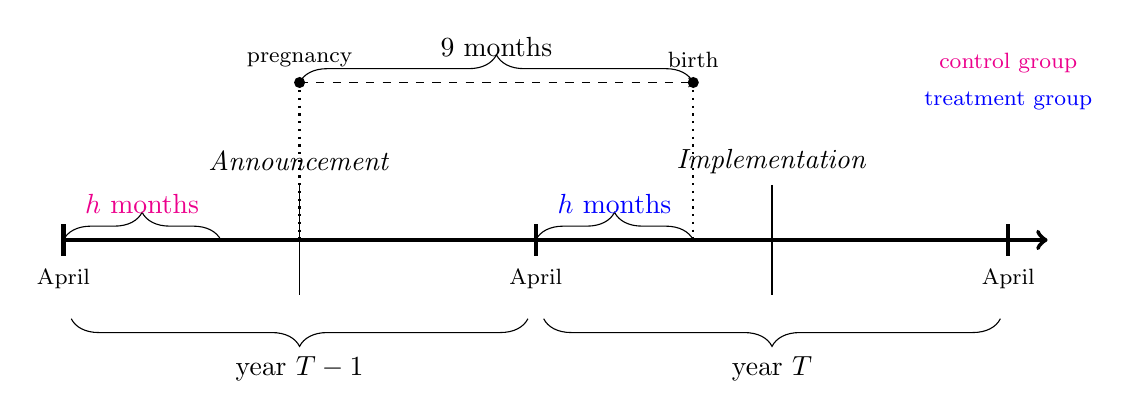
\begin{tikzpicture}

  % Draw the main timeline
  \draw[->,ultra thick] (0,0) -- (12.5,0);
  % \draw[->] (0,3) -- (18,3);
  
  % Annotations on the top line
  \node at (3, 3.5-2-0.5) {\textit{Announcement}};
  \node at (9, 3.5-2-0.5) {\textit{Implementation}};
  % \draw (3,3.2) -- (3,2.8);
  % \draw (9,3.2) -- (9,2.8);
  \draw (3,3.2-2-0.5) -- (3,2.8-3-0.5);
  \draw (9,3.2-2-0.5) -- (9,2.8-3-0.5);
  
  % Pregnant and birth labels on the top line
  \node[above,yshift=2pt] at (3, 2.5-0.5) {\footnotesize pregnancy};
  \node[above,yshift=2pt] at (8, 2.5-0.5) {\footnotesize birth};
  \draw[decorate, decoration={brace, amplitude=10pt}] (3,2) -- (8,2) node[midway, above,yshift=6pt] {9 months};
  % \node[above,yshift=2pt] at (9, 2.5-0.5) {pregnancy};
  % \node[above,yshift=2pt] at (14, 2.5-0.5) {birth};
  % \draw[decorate, decoration={brace, amplitude=10pt}] (9,2) -- (14,2) node[midway, above,yshift=6pt] {9 months};
  \fill (3, 2.5-0.5) circle (2pt);
  \fill (8, 2.5-0.5) circle (2pt);
  % \fill (9, 2.5-0.5) circle (2pt);
  % \fill (14, 2.5-0.5) circle (2pt);
  \draw[->,dashed] (3, 2.5-0.5) -- (8, 2.5-0.5);
  % \draw[->,dashed] (9, 2.5-0.5) -- (14, 2.5-0.5);
  \draw[dotted,thick] (8, 2.5-0.5) -- (8, 0);
  % \draw[dotted,thick] (14, 2.5-0.5) -- (14, 0);
  \draw[dotted,thick] (3, 2.5-0.5) -- (3, 0);
  % \draw[dotted,thick] (9, 2.5-0.5) -- (9, 0);

  \draw[decorate, decoration={brace, amplitude=10pt}] (0,0) -- (2,0) node[midway, above,yshift=6pt,magenta] {$h$ months};
  \draw[decorate, decoration={brace, amplitude=10pt}] (6,0) -- (8,0) node[midway, above,yshift=6pt,blue] {$h$ months};
  % \draw[decorate, decoration={brace, amplitude=10pt}] (12,0) -- (14,0) node[midway, above,yshift=6pt] {$h$ months};
  \node[above,magenta] at (12,2) {\footnotesize control group};
  \node[below,blue] at (12,2) {\footnotesize treatment group};
  
  % Lower timeline labels
  \node at (0, -0.5) {\footnotesize April};
  \node at (6, -0.5) {\footnotesize April};
  \node at (12, -0.5) {\footnotesize April};
  \draw[ultra thick] (0, 0.2) -- (0, -0.2);
  \draw[ultra thick] (6, 0.2) -- (6, -0.2);
  \draw[ultra thick] (12, 0.2) -- (12, -0.2);
  
  % Labels for cohort periods
  \draw[decorate, decoration={brace, amplitude=10pt, mirror}] (0.1,-1) -- (5.9,-1) node[midway, below,yshift=-10pt] {year $T-1$};
  \draw[decorate, decoration={brace, amplitude=10pt, mirror}] (6.1,-1) -- (11.9,-1) node[midway, below,yshift=-10pt] {year $T$};
  % \draw[decorate, decoration={brace, amplitude=10pt, mirror}] (12.1,-1) -- (17.9,-1) node[midway, below,yshift=-10pt] {year $T+1$};
  
  \end{tikzpicture}
}
  \caption{Timeline}
  \label{fig:timeline}
\end{figure}

I assume that it takes at least nine months from pregnancy to childbirth.
This is because around 95\% of children are born more than nine months after pregnancy in Japan (\cite{sakata2018}).
Also, suppose the lag is one year between the announcement and the implementation.
Then, I denote a fiscal year as year $T$ if the year contains the date of nine months after the announcement.
I also denote a year before year $T$ as year $T-1$, a year after year $T$ as year $T+1$, and so on.
Figure \ref{fig:timeline} shows the case where the announcement is made later than May, but the classification holds for any month of the announcement.


Then, see the mothers whose first child is born in year $T-1$. 
All of these mothers are pregnant ``before'' the announcement, so none of them are affected by the announcement.
Also, see the mothers whose first child was born in the year $T$. 
Then, mothers whose first child is born in the first some months (denote as $h$ months) are pregnant ``before'' the announcement, and the others are pregnant ``after'' the announcement.
As a result, due to the postponement of marriage and pregnancy I explained above, the number of first children born in year $T$ is expected to be smaller than that in year $T-1$.


Based on the argument above, I classify the mothers whose first child is born in the first $h$ months in year $T$ as the treatment group and the mothers whose first child is born in the first $h$ months in year $T-1$ as the control group (see Figure \ref{fig:timeline}).
Then, it is plausible to expect that the distribution of predetermined characteristics of mothers is identical between the treatment and control groups\footnote{I can partially test this by balancing test.}.
Both do not know the policy when deciding on pregnancy, and their childbirths differ only by a year.
The only difference is the number of coetaneous children. 
Compared to the control group, the treatment group has fewer coetaneous children due to the postponement of marriage and pregnancy.
This reduction in the coetaneous children leads to better access to childcare services. 
Mothers in the treatment group have better access to childcare services because there is less demand and more availability. 
Therefore, mothers in the treatment group can be regarded as randomly assigned to the treatment, which assigns childcare service with imperfect compliance\footnote{Mothers are not forced to use childcare service, so compliance is incomplete.}.


Note that the control group is restricted to the first $h$ months in year $T-1$, not the whole year.
This is because of the seasonality of childbirth: the characteristics of mothers differ by the season of childbirth\cite{Buckles2013-tj}. 
To eliminate the effect of seasonality, I restrict the sample to the first $h$ months in year $T-1$ and year $T$.

\subsection*{Regression Formulation}
Let $Y_i^s$ be the labor supply of mother $i$ when her first child is $s$ years old, such as working hours, labor force participation, earnings, etc.
Also, let $D_i^s$ be the indicator of whether mother $i$ uses childcare service. 
Then, the causal relationship of interest is 
\begin{equation}
  Y_i^s = \alpha + \beta D_i^s + \vb{X}_i'\vb{\gamma} + \epsilon_i, \label{step2}
\end{equation}
where $\vb{X}_i$ is the vector of predetermined characteristics of mother $i$, such as education, birth-month of the child, husband's income, etc.
$s$ can be 1, 2, 3, and so on.


In the equation \eqref{step2}, $\beta$ is the treatment effect of childcare service on mothers' labor supply.
However, na\"ive OLS returns the biased estimate of $\beta$ because mothers who use childcare services are likely to be more enthusiastic about working.
To deal with this endogeneity, I formulate the first stage estimation as follows:
\begin{equation}
  D_i^s = \varphi + \pi Z_i + \vb{X}_i'\vb{\delta} + \eta_i, \label{step1}
\end{equation}
where $Z_i$ is the indicator of whether mother $i$ is in the treatment group.
By estimating \eqref{step2} and \eqref{step1} by 2SLS, I can obtain the unbiased and consistent estimate of $\beta$. 

\subsection*{Validation of Identification Strategy}
In this subsection, I validate the instrumental variable $Z_i$.
First, relevance is expected to hold, i.e., $Z_i$ is correlated with $D_i^s$ strongly enough. 
As \cite{nhk} shows, a large fraction of Japanese people support the introduction of optional separate surnames, and the fraction is larger in the younger generation.
In addition, the cost of choosing separate surnames is lower for couples who marry after the implementation than for those who marry before the implementation and already share the same surname.
Therefore, it is plausible to expect that the number of those choosing separate surnames and postponing marriage is not small. 
In addition, according to the Specified Report of Vital Statistics in 2021 by the Ministry of Health, Labour and Welfare, more than 80\% of couples get pregnant with their first child after marriage.
Therefore, a significant number of postponements of pregnancies are expected due to the postponement of marriage, which results in the considerable reduction of coetaneous children.


Second, the exclusion restriction is expected to hold, i.e., $Z_i$ affects $Y_i^s$ only through $D_i^s$.
As explained above, the distribution of predetermined characteristics of mothers is identical between the treatment and control groups, both observable and unobservable.
Therefore, whether mother $i$ is assigned to the treatment or control group does not affect $Y_i^s$ except through $D_i^s$.
The only possibility of violating the exclusion restriction is the difference in the announcement's timing. 
For mothers in the treatment group, the announcement is made when they are pregnant, while for mothers in the control group, the announcement is made when they are not pregnant.
The exclusion restriction is violated if this difference directly affects mothers' labor supply.
However, I expect this is unlikely because the announcement is not directly related to mothers' labor supply.
The only one-year difference in the announcement's timing is unlikely to affect mothers' labor supply.

\section{Data}
A cross-sectional dataset is required to conduct the empirical analysis.
I enumerate the necessary variables below: 
\begin{description}
  \item[Outcome Variable] mothers' labor supply \\ 
  Either of the working hours, working days, labor force participation, earnings, employment status, etc.
  \item[Treatment Variable] use of childcare service of mother's first child 
  \item[Instrumental Variable] birth month of mother's first child
  \item[Other Control Variables] predetermined characteristics of mother \\
  mother's education, age, working experience, husband's income, children's gender, whether grandparents live together, etc.
\end{description}
The first three variables are indispensable for estimation. 


The first choice of the dataset is Comprehensive Survey of Living Conditions\footnote{See \url{https://www.mhlw.go.jp/toukei/list/20-21.html} for detail.}, which is conducted by the Ministry of Health, Labour and Welfare.
This survey is conducted yearly, and once every three years, a large-scale survey is conducted.
This large-scale survey contains all the information necessary for the estimation.
For example, it contains each household member's demographic and social information, such as gender, birth year and month, education, earnings, working days and hours, employment status, working experience, etc.
In addition, if they have children of preschool age, I can see how they are taken care of: by parents, grandparents, accredited childcare services, non-accredited childcare services, kindergarten, etc. 
As a result, I can estimate the treatment effect in detail, considering the type of childcare service.


The number of observations in the dataset is around 300,000 households and around 700,000 individuals in the large-scale surveys.
According to Vital Statistics and Comprehensive Survey of Living Conditions, in 2022, there were 504,930 marriages, while the number of households was about 54,310,000. 
Roughly estimated, about 1\% of households are married in a year.
Therefore, 3,000 households could be the treatment or control groups in one year of the survey. 
In addition, since the survey changes the sample every year, I can obtain more observations by pooling the data from multiple years.


The questionnaire data of the Comprehensive Survey of Living Conditions can be used for research purposes\footnote{
  I can use the data for free if I have Kakenhi. 
  See miripo for details: \url{https://www.e-stat.go.jp/microdata/data-use}.
}.
In sum, I can obtain the necessary dataset with enough sample size and information, and this proposal is feasible if optional separate surnames are implemented in Japan.


Although the dataset above is expected to be enough, tax data from CREPE (Center for Research and Education in Program Evaluation) at the University of Tokyo is another candidate.
As a project to promote EBPM, they collect tax data from endorsing municipalities and construct a dataset. 
The strength of the dataset is its sample size: \cite[Kondo and Fukai]{kondo2023} use the dataset, and its sample size for married women is more than 3,000,000. 
However, it lacks information on the use of childcare services. 
\cite{kondo2024} combines the dataset with the administrative data of accredited childcare services, but the data is not available to the public, so it is unclear whether I can use the data or not.
Therefore, the first choice is the Comprehensive Survey of Living Conditions.



\nocite{*}
\bibliography{research_proposal}
\bibliographystyle{econ}

\end{document}